%This document was modified by Asst Prof Adriana Lopes from the latex template "NTU CNYSP Research Report Template (CY1400-CY2001-CY2002)" authored by Karn Watcharasupat.  This is a simplified version to be used by ASE students during their FYP. 


%\documentclass{article}
%\documentclass[12pt,twoside,openright]{report} - with white page between major sections
\documentclass[12pt]{report}

%% Useful packages
\usepackage[a4paper,top=1in,bottom=1in,left=1in,right=1in]{geometry}
\usepackage{amsmath, amssymb, bm}
\usepackage{caption}
\usepackage{graphicx}
\usepackage[colorinlistoftodos]{todonotes}
\usepackage[colorlinks=true, allcolors=black]{hyperref}
\usepackage{float}
\usepackage{setspace}
\usepackage{subfigure}
\usepackage{url}
\usepackage{tabularx}
\usepackage[utf8]{inputenc}
\usepackage{mathptmx} %Times Font
\usepackage{titlesec}
\titlespacing{\chapter}{0pt}{0pt}{0pt}
\usepackage{fancyhdr}
\usepackage{etoolbox}
\usepackage{appendix}
\usepackage{siunitx}
\usepackage{nomencl}
\newcommand{\nomunit}[1]{%
	\renewcommand{\nomentryend}{\hspace*{\fill}#1}}
\makenomenclature
\usepackage{caption}
\usepackage{lipsum}
\usepackage{algpseudocode}
\usepackage{empheq}
\usepackage{mdwlist}
\usepackage{booktabs}
\usepackage{colortbl}
\widowpenalty 10000
\clubpenalty 10000
\usepackage{moresize}

\usepackage[style=apa]{biblatex}
\addbibresource{References.bib}
\DeclareSourcemap{
	\maps[datatype=bibtex]{
		\map{
			\step[fieldsource=title, match=\regexp{\b([A-Z]{2,})\b}, replace={{}{$1}}]
		}
	}
}

\DeclareCaptionType{appfigure}[Figure]
\DeclareCaptionType{apptable}[Table]
\renewcommand{\listappfigurename}{List of Appendix Figures}
\renewcommand{\listapptablename}{List of Appendix Tables}
\renewcommand{\thefigure}{\thechapter-\arabic{figure}}
\renewcommand{\thetable}{\thechapter-\arabic{table}}
\renewcommand{\theappfigure}{\thechapter-\arabic{appfigure}}
\renewcommand{\theapptable}{\thechapter-\arabic{apptable}}
\renewcommand{\contentsname}{Table of Contents}

\newcommand{\chapname}{Chapter }

\titleformat{\chapter}[block]
{\bfseries\LARGE\centering}
{}{1em}{}[\rule{\textwidth}{0.3pt}]

\titleformat{\section}
{\bfseries\large}
{\thesection}{1em}{}

\titleformat{\subsection}
{\normalfont\bfseries}
{\thesubsection}{1em}{}

\titleformat{\subsubsection}
{\normalfont\bfseries}
{\thesubsubsection}{1em}{}

\usepackage{fancyhdr}
\usepackage{multirow}
\usepackage{multicol}

\usepackage{placeins}

\makeatletter
\renewcommand*\env@matrix[1][*\c@MaxMatrixCols c]{%
	\hskip -\arraycolsep
	\let\@ifnextchar\new@ifnextchar
	\array{#1}}
\makeatother

\usepackage{enumitem}

\usepackage{listings}
\usepackage{color}

\definecolor{codegreen}{rgb}{0,0.6,0}
\definecolor{codegray}{rgb}{0.5,0.5,0.5}
\definecolor{codepurple}{rgb}{0.58,0,0.82}
\definecolor{backcolour}{rgb}{0.95,0.95,0.95}

\newcommand{\codesize}{\fontsize{10pt}{11pt}\selectfont}

\lstdefinestyle{mystyle}{
	backgroundcolor=\color{backcolour},   
	commentstyle=\color{codegreen},
	keywordstyle=\color{magenta},
	numberstyle=\tiny\color{codegray},
	stringstyle=\color{codepurple},
	basicstyle=\ttfamily\codesize,
	breakatwhitespace=true,         
	breaklines=true,                 
	captionpos=b,                    
	keepspaces=false,                 
	numbers=left,                    
	numbersep=5pt,                  
	showspaces=false,                
	showstringspaces=false,
	showtabs=false,                  
	tabsize=2,
	showlines = true,
	fontadjust = true,
	framexleftmargin = 10 pt,
	resetmargins = true,
	basewidth = 0.5em
}

\lstset{style=mystyle}

\makeatletter
\setlength{\@fptop}{0pt}
\makeatother

\setlength{\floatsep}{0pt}

\newenvironment{Figure}
{\noindent\minipage{\linewidth}}
{\endminipage}

\setcounter{secnumdepth}{5}

\hyphenpenalty 10000
\usepackage{multicol}

%%%%%%%%% MATHEMATICS SHORTHANDS %%%%%%%%%%%%%%%%%%%% 

\newcommand{\C}{\mathbb{C}}
\newcommand{\R}{\mathbb{R}}
\newcommand{\Z}{\mathbb{Z}}
\renewcommand{\d}{\mathrm{d}}
\renewcommand{\bf}[1]{\mathbf{#1}}

\newcommand{\argmax}[1]{\underset {#1}{\operatorname{arg\,max}}}

\newcommand{\kurt}{\mathrm{kurt}}
\newcommand{\round}{\operatorname{round}}

\newcommand{\E}{\operatorname{E}}
\newcommand{\cov}{\operatorname{cov}}
\newcommand{\pcov}{\operatorname{pcov}}

\newcommand*{\vertbar}{\rule[-1ex]{0.5pt}{2.5ex}}
\newcommand*{\horzbar}{\rule[.5ex]{2.5ex}{0.5pt}}

\setlength{\nomlabelwidth}{3cm}
\setlength{\nomitemsep}{-0.5\parsep}

\usepackage{makecell}
\usepackage{emptypage}
\usepackage{booktabs}

\newcolumntype{R}{>{\raggedleft\arraybackslash}X}
\newcolumntype{L}{>{\raggedright\arraybackslash}X}
\newcolumntype{C}{>{\centering\arraybackslash}X}

\usepackage{textcomp}

%
%\usepackage{background}

%\SetBgScale{1}
%\SetBgContents{\parbox{10cm}{%
		%  \Huge Draft:  \today\\[14cm]\rotatebox{180}{\Huge Draft:  %\today}}}
%\SetBgColor{gray}
%\SetBgAngle{270}
%\SetBgOpacity{0.1}
%

%%%%%%%%%%%%%%%%%%%%%%%%%%%%%%%%%%%%%%%%%%%%%%%%%%%%%
\begin{document}
	\sloppy
	%==== FRONT PART====
	\begin{titlepage}
	\begin{figure}[!t]
		\centering
		
\includegraphics[width = 4.3in]{title/logo.pdf}
		\caption*{}
	\end{figure}
	
	\centering
	\LARGE{\textbf{SC2207: Introduction to Databases}}\\[0.2in]
	\LARGE{\textbf{Lab 1 Report}}\\[1.5in]
	
%	\LARGE{\textbf{YOUR NAME}}\\
%	\normalsize{Matriculation number}\\[0.2in]

	\begin{table}[h]
		\centering
		\begin{tabular}{lll}
			\toprule
			\textbf{Name} & \textbf{Email} & \textbf{Matric Number} \\
			\midrule
			Pu Fanyi & FPU001@e.ntu.edu.sg & U2220175K \\
			Jin Qingyang & JINQ0003@e.ntu.edu.sg & U2220239A \\
			Tang Yutong & TANG0513@e.ntu.edu.sg & U2220495H \\
			Ye Yuhan & YYE016@e.ntu.edu.sg & U2220885J \\
			Ting Ruo Chee & RTING002@e.ntu.edu.sg & U2220572C \\
			Soo Ying Xi & D220001@e.ntu.edu.sg & U2220021D \\
			Qian Jianheng Oscar & QIAN0081@e.ntu.edu.sg & U2220109K \\
			\bottomrule
		\end{tabular}
%		\caption{List of Names, Emails, and Matric Numbers}
%		\label{tab:my-table}
	\end{table}

	\large{Tutorial Group: SCSD}\\
	\large{Lab Supervisor: Sourav Saha Bhowmick}\\
	\large{Teaching Assistant: Yu Weiping}\\[0.5in]
	
%	\large{A Final Year Report submitted to Asian School of the Environment, Nanyang Technological University in partial fulfilment of the requirements for the Degree of }\\[0.1in]
	
	\Large{School of Computer Science and Engineering}\\
	\Large{Nanyang Technological University}\\[0.3in]
	
	
	\Large{2023/2024 Semester 2}
	\newpage
\end{titlepage}
	\newpage
	%=== FRONT PART ===
%=== ABSTRCT ===

%\begin{center}
\chapter*{ER Diagram}
%\rhead{Abstract}
%\end{center}
\addcontentsline{toc}{chapter}{Abstract}

\begin{center}
	\makebox[\textwidth]{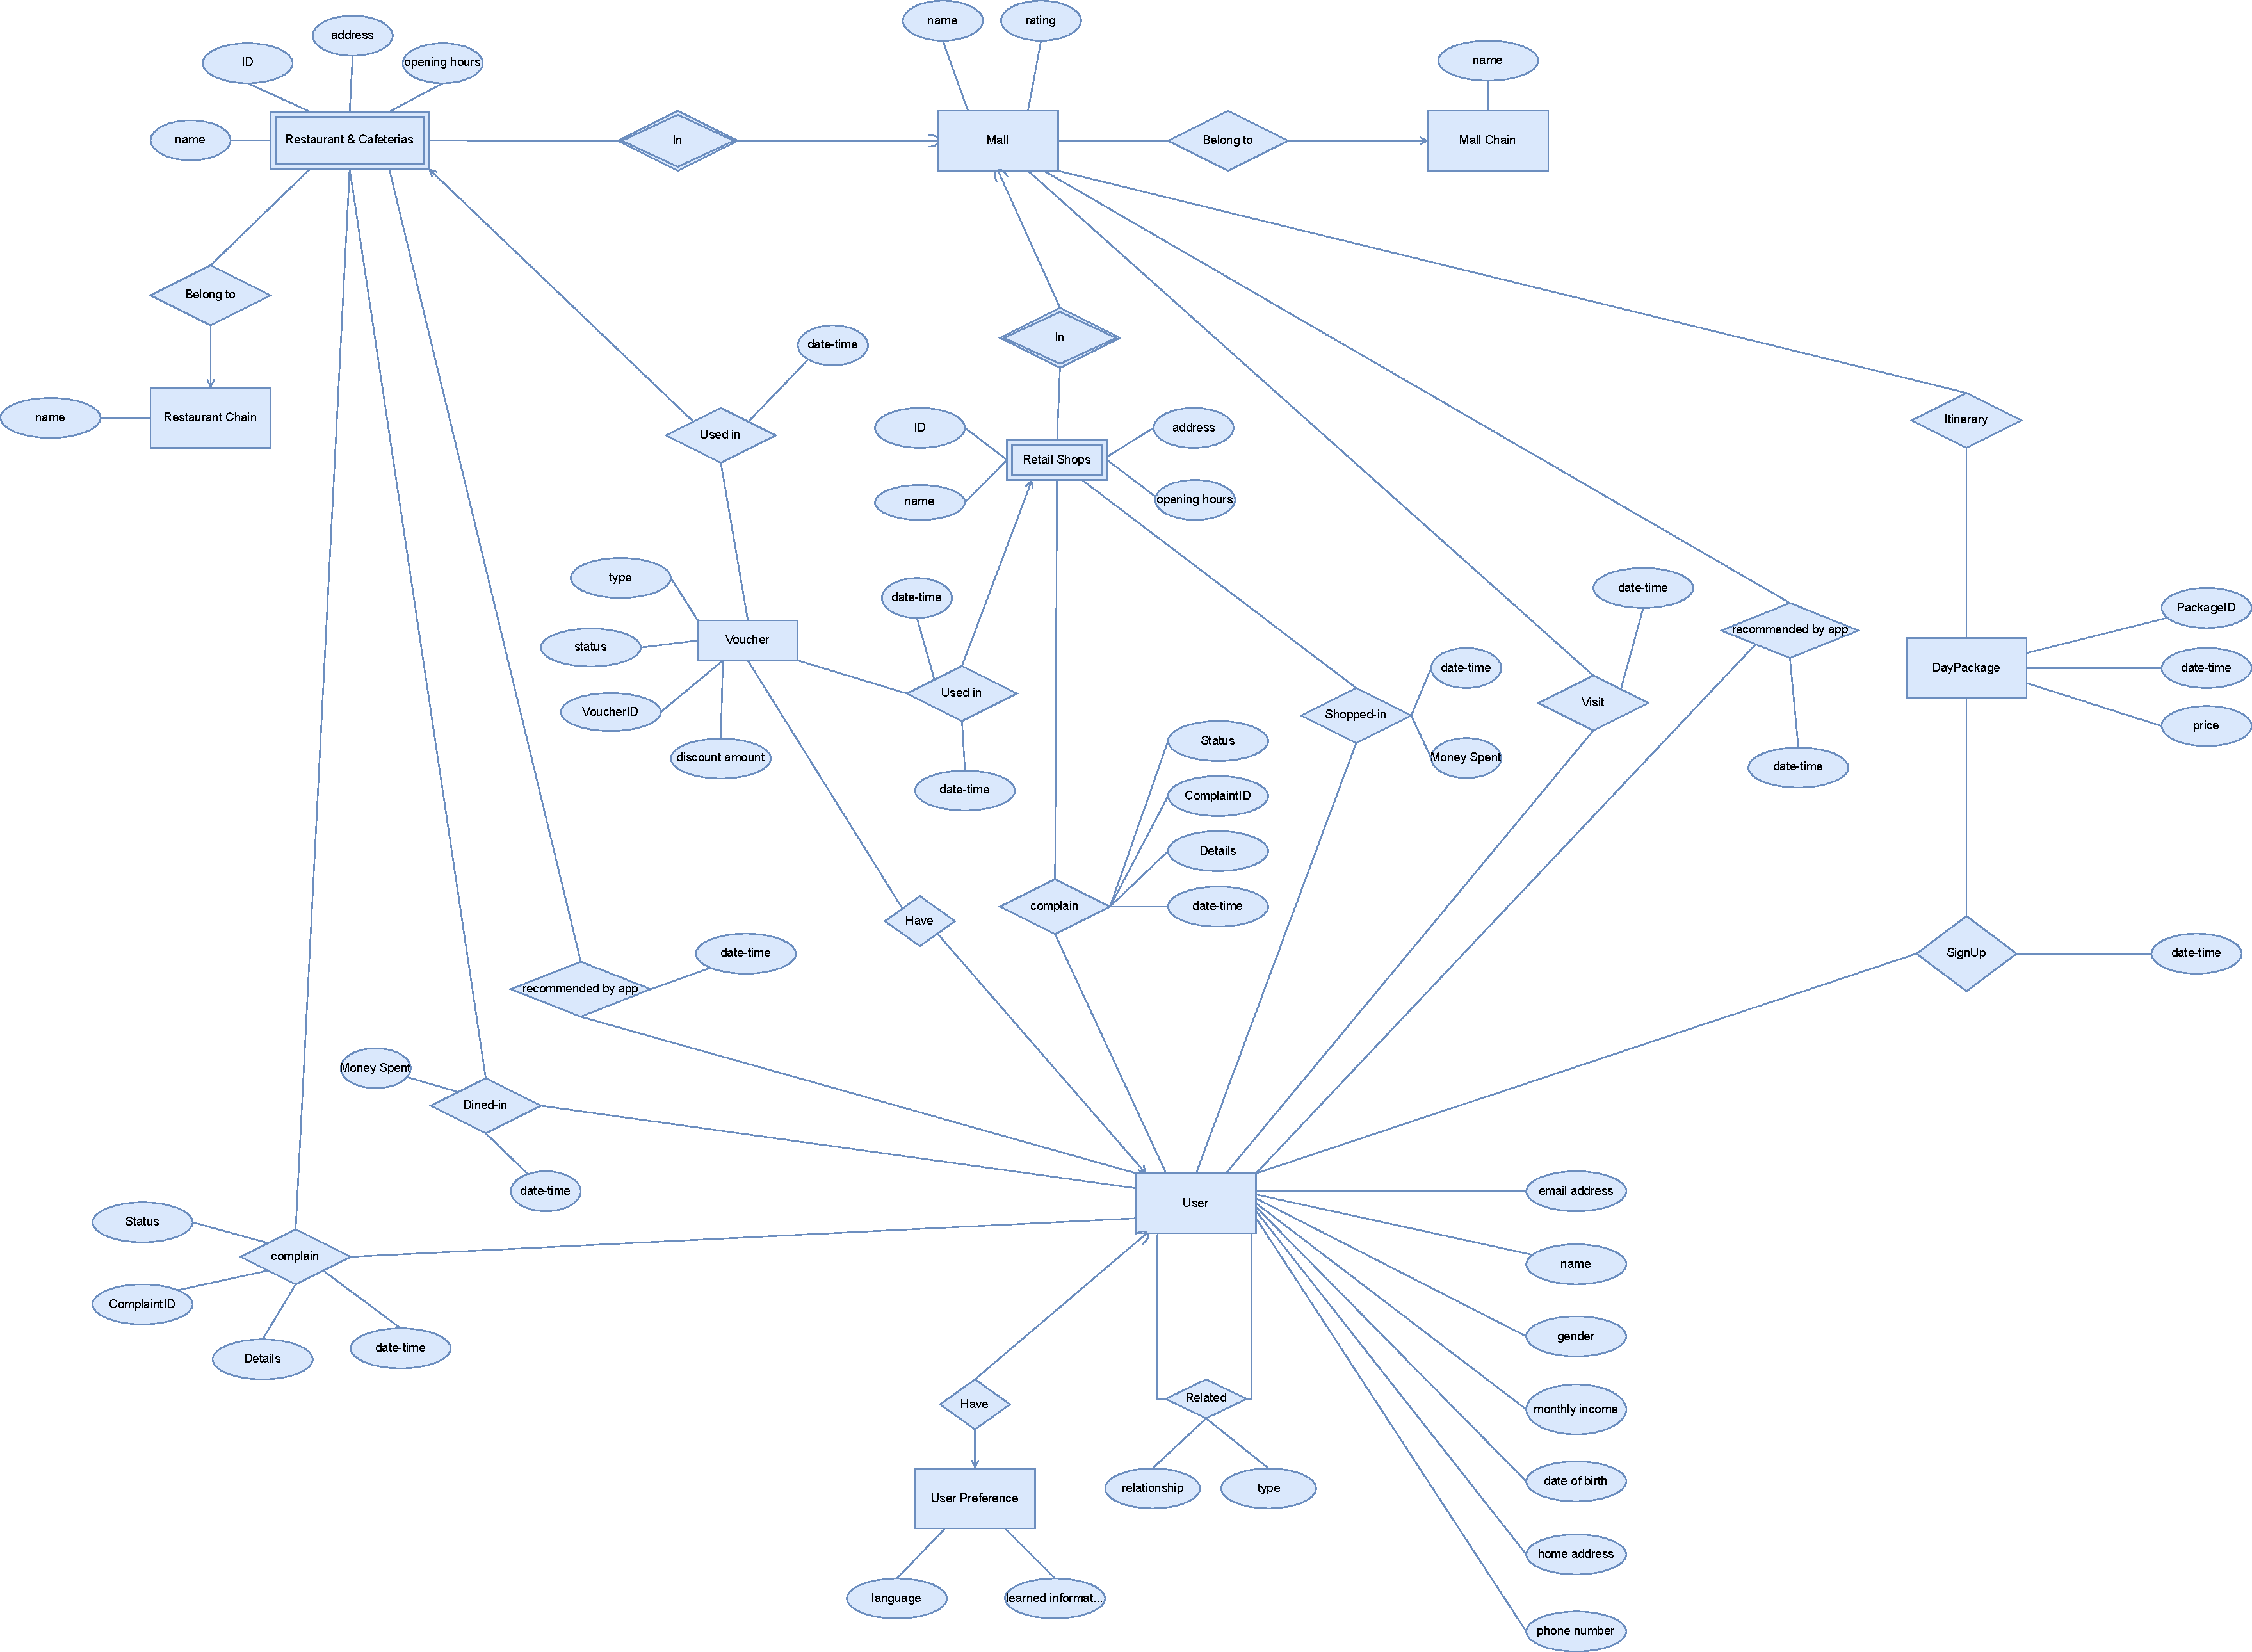
\includegraphics[width=\textwidth]{diagram/Lab1.pdf}}
\end{center}

	\newpage
	%=== FRONT PART ===
%=== ABSTRCT ===

%\begin{center}
\chapter*{Explanations}
%\rhead{Abstract}
%\end{center}
\addcontentsline{toc}{chapter}{Abstract}

Write something...

	\newpage
	%=== FRONT PART ===
%=== ABSTRCT ===

%\begin{center}
\chapter*{Individual Contribution Form}
%\rhead{Abstract}
%\end{center}
\addcontentsline{toc}{chapter}{Abstract}


\begin{center}
	\makebox[\textwidth]{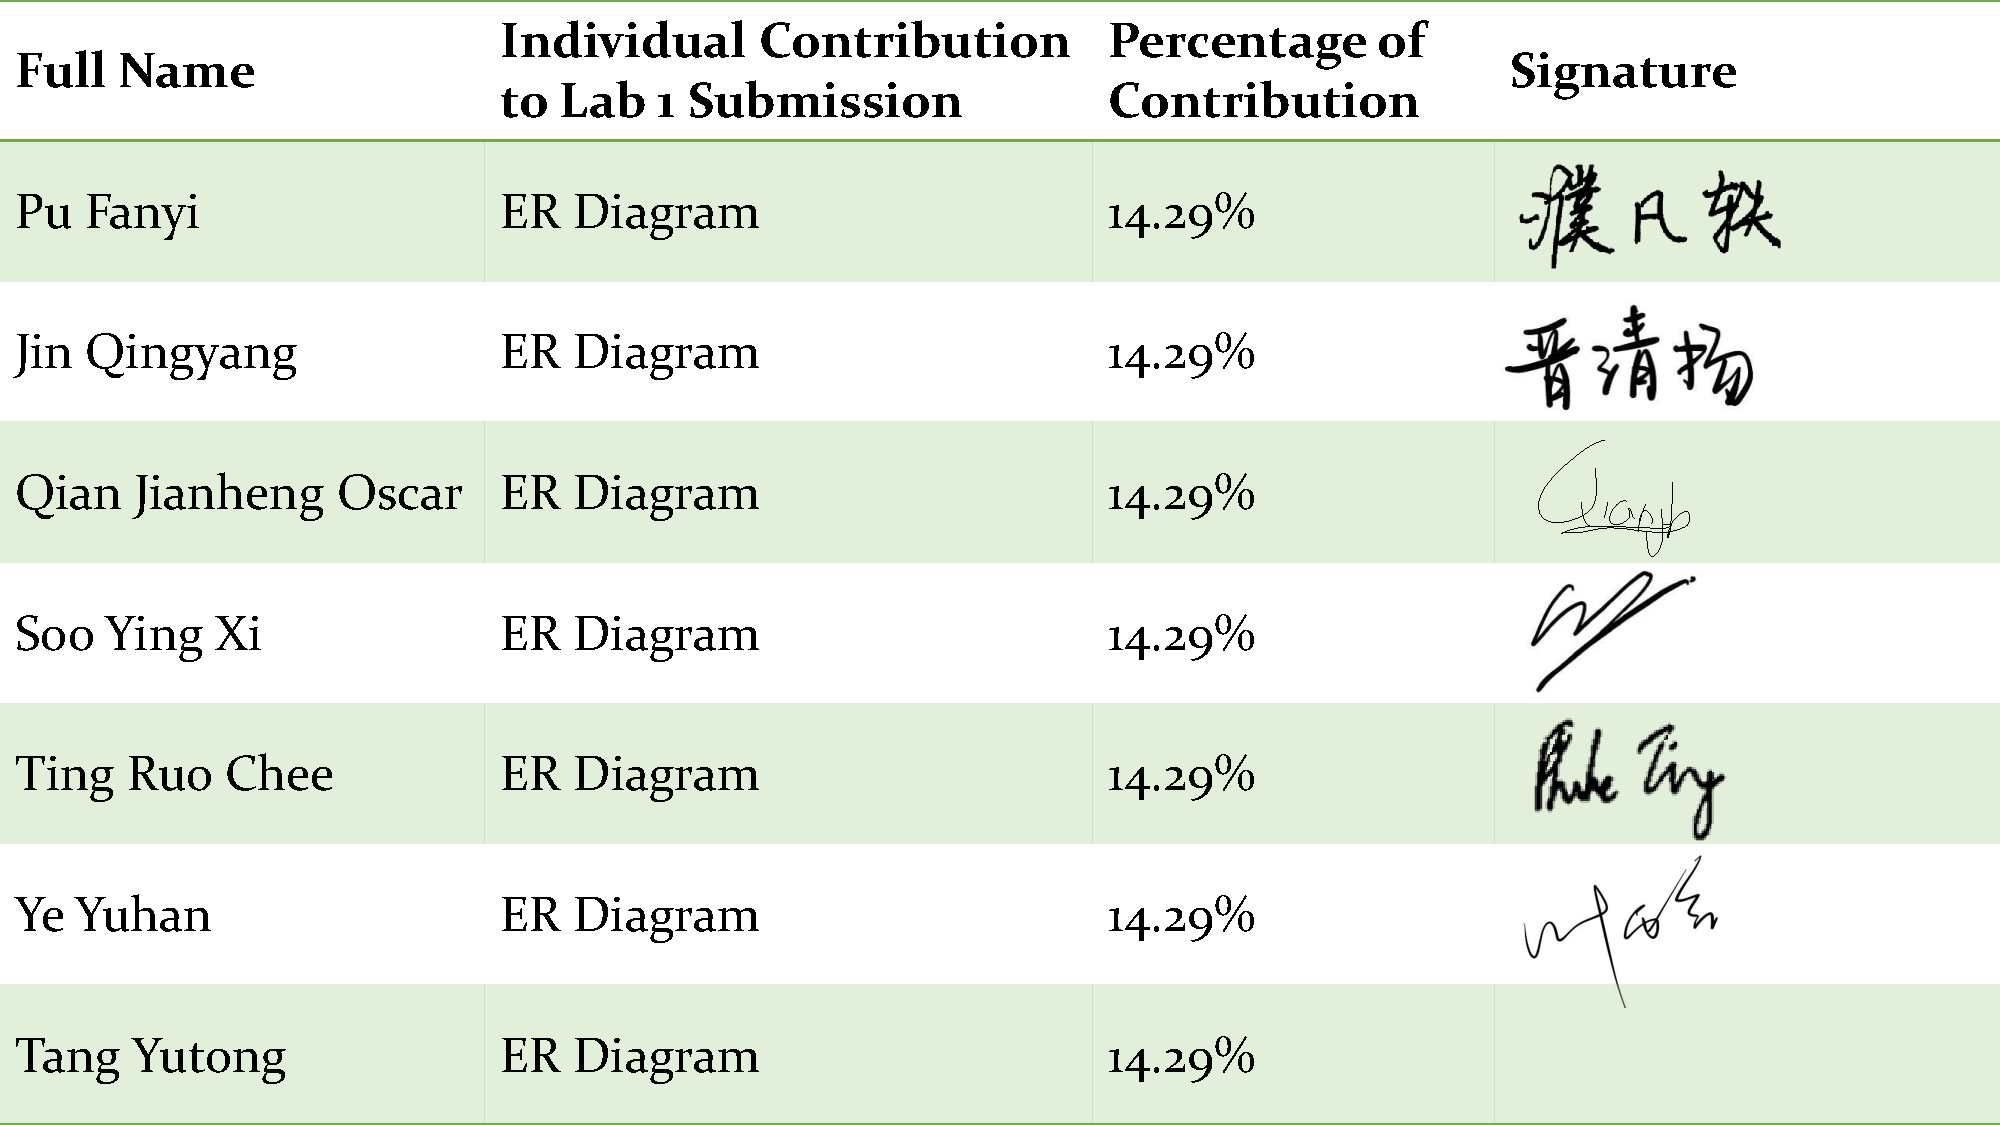
\includegraphics[width=\textwidth]{appendix/form.pdf}}
\end{center}


	
%	%\begingroup
%	%\let\cleardoublepage\clearpage
%	\pagenumbering{roman}
%	\pagestyle{fancy}
%	\fancyhf{}
%	\cfoot{\thepage}
%	%\endgroup
%	
%	\include{Front/Abstract}
%	\newpage
%	
%	\include{Front/Graphical_Abstract}
%	\newpage
%	
%	\include{Front/Acknowledgement}
%	\newpage
%	\setcounter{tocdepth}{2}
%	
%	\tableofcontents
%	\rhead{Table of Contents}
%	\newpage
%	
%	%\include{Front/Nomenclature}
%	%\newpage
%	
%	\renewcommand{\listfigurename}{Lists of Figures}
%	\rhead{Lists of Figures}
%	\listoffigures 
%	\addcontentsline{toc}{chapter}{Lists of Figures}
%	
%	\newpage
%	
%	
%	\listoftables 
%	\addcontentsline{toc}{chapter}{Lists of Tables}
%	\rhead{Lists of Tables}
%	\newpage
%	
%	\rhead{}
%	
%	%==== MAIN PART ====
%	\pagenumbering{arabic}
%	\lhead{Introduction}
%	\include{Introduction/Introduction}
%	\lhead{Material and Methods}
%	\include{Material_and_Methods/MM}
%	\lhead{Results and Discussion}
%	\include{Results_and_Discussion/Results_and_Discussion}
%	\lhead{Conclusion and Future Work}
%	\include{Conclusion/Conclusion}
%	\addcontentsline{toc}{chapter}{References} % see https://tex.stackexchange.com/questions/119719/add-an-item-in-the-table-of-contents
%	\printbibliography[title={References}]
%	
%	%==== ENDING PART ===
%	\clearpage
%	\pagenumbering{arabic}%
%	\renewcommand{\thepage}{R-\arabic{page}}
%	\lhead{}
%	%\rhead{References}
%	%\printbibliography[title={References}]
%	
%	%=================================
%	\newpage
%	\appendix
%	\renewcommand{\chapname}{Appendix}
%	\pretocmd{\chapter}{%
%		\clearpage
%		\pagenumbering{arabic}%
%		\renewcommand*{\thepage}{\thechapter-\arabic{page}}%
%	}{}{}
%	\rhead{Appendix}
%	%\lhead{Source Information}
%	\include{Appendix/Appendix}
%	%==== END OF ALL ===
\end{document}
